\documentclass[a4paper,12pt]{report}
\usepackage[margin=1.5cm]{geometry}
\usepackage[utf8]{inputenc}
\usepackage[french]{babel}
\usepackage{graphicx}
\graphicspath{ {figures/} }

\title{Rapport de stage M2 \\ Working Title}
\author{Gaël Touquet}

\begin{document}

\maketitle
\newpage
\tableofcontents

\addcontentsline{toc}{chapter}{Introduction}
\chapter*{Introduction}

à bosser

\chapter{Cadre théorique : le modèle standard des particules}

-les particules, les interactions , etc

% insister sur le caractère stable/instable des particules et leur detectabilité

\chapter{Cadre experimental : collisionneurs et detection}

L'amélioration du modèle théorique passe par la réalisation d'experience procurant des informations sur les propriétés des consistuants fondamentaux que sont les particules. Ainsi des expériences de type $collisionneurs$ ont vu l'aube dans le but de produire les-dites particules de manière relativement isolées. Puis des experiences de détections permettent de récupérer les informations permettant de remonter aux caractéristiques de celles-ci .

\section{Les collisionneurs}

Le principe des collisionneurs réside dans la notion de transformation de l'énérgie cinétique sous forme d'énergie de masse d'après la formule:

\begin{equation}
\label{Energie}
E^{2} = p^{2}c^{2} + m^{2}c^{4}
%\caption{ici $p^{2}c^{2}$ représente l'energie cinétique et $m^{2}c^{4}$ est l'énérgie de masse}
\end{equation}


Ainsi la conservation de l'énergie totale n'empéche pas de transformer de l'énergie sous forme cinétique en énergie sous forme de masse, c'est à dire fabriquer des nouvelles particules de matières.

Pour ce faire la partie accélérateur du collisioneur va fournir de l'énergie à des paquets de particules relativement communes isolées préalablement. Ces particules peuvent être soit fondamentales (electron, positron) soit composites (proton ou plus généralement hadron). Differents paquets de particules vont être amenés à se rencontrer face à face de manière à ce que l'impulsion totale des deux particules incidentes dans le référentiel du laboratoire soit nulle.
%voir s'il n'est pas possible de mettre une référence à propos des differents types de projets de collisioneurs : ee ou pp

Ces particules accélérées vont ensuite collisionner %TODO

\section{La detection}

De nombreuses particules sont donc issues d'une collision et ces particules peuvent 

\begin{figure}[h]
\caption{Schéma de coupe du détecteur CMS}
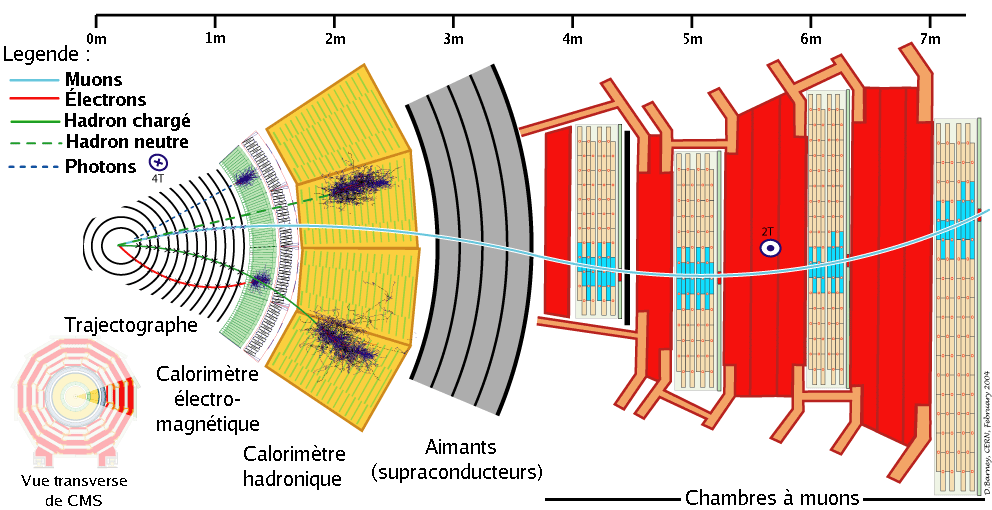
\includegraphics[width=\textwidth]{Schema_transverse_cms}
\label{CMScouches}
\end{figure}

\paragraph{L'aimant} n'est pas un sous-detecteur en soit mais il permet de maintenir un champ magnétique constant dans le 

\chapter{L'algorithme de particle-flow}
%introduire la reconstruction à partir des traces et clusters

\section{Le principe du particle flow}
%on détaille ce que fait le particle flow de manière générale cad reconstruction des p4 et id des particules par étape et analyse des ensembles de traces et clusters



\end{document}
